% !TeX root
\documentclass[12pt]{report}

% includes
\usepackage{geometry}           % page size
\usepackage[utf8]{inputenc}     % encoding
\usepackage{palatino}           % font
\usepackage[romanian]{babel}    % language
\usepackage{graphicx}           % images
\usepackage{indentfirst}        % indentation
\usepackage[nottoc]{tocbibind}  % table of contents style
\usepackage[unicode]{hyperref}  % references from the table of contents
\usepackage{wrapfig}			% image wrapping
\usepackage{subcaption}			% row  image positioning
\usepackage{listings}			% used for code showcase
\usepackage{multicol}			% multi-column support for itemize env
\usepackage{color}				% for color suport
% includes options
\geometry{  a4paper,            % scientific thesis standard
            left=3cm,
            right=2cm,
            top=2cm,
            bottom=2cm,
 }
\graphicspath{{images/}}        % path where the images are located
\setlength{\parindent}{1cm}     % paragraph indentation

% other options
\linespread{1.5}                % space between lines
\renewcommand*\contentsname{Cuprins}    % table of contents name

% set the style for code
\definecolor{codegreen}{rgb}{0,0.6,0}
\definecolor{codegray}{rgb}{0.5,0.5,0.5}
\definecolor{codepurple}{rgb}{0.58,0,0.82}
\definecolor{codeyellow}{rgb}{0.67,0.67,0.0}
\definecolor{backcolour}{rgb}{0.95,0.95,0.92}

\lstdefinestyle{python}{
	language=Python,
	basicstyle=\ttfamily\footnotesize,
	backgroundcolor=\color{backcolour},   
	commentstyle=\color{codegreen},
	keywordstyle=\color{magenta},
	emph={testfunc,print,src},
	emphstyle=\color{codeyellow},
	numberstyle=\tiny\color{codegray},
	stringstyle=\color{codepurple},
	breakatwhitespace=false,         
	breaklines=true,                 
	captionpos=b,                    
	keepspaces=true,                 
	numbers=left,                    
	numbersep=5pt,                  
	showspaces=false,                
	showstringspaces=false,
	showtabs=false,                  
	tabsize=2
}

% the document content
\begin{document}
    % macros (global)
    \newcommand{\university}    {Universitatea "Alexandru-Ioan Cuza" din Iași}
\newcommand{\universityg}   {Universității "Alexandru-Ioan Cuza" din Iași} % genitive
\newcommand{\faculty}       {Facultatea de informatică}
\newcommand{\facultyg}      {Facultății de informatică} % genitive
\newcommand{\speciality}    {informatică}
\newcommand{\promotion}     {2023}                                  %<---------

\newcommand{\thesistype}    {Lucrare de licență}
\newcommand{\thesistitle}   {Home Smartup}    %<---------

\newcommand{\authorlast}    {Petrache}                               %<---------
\newcommand{\authorfirst}   {Liviu-Andrei}
\newcommand{\authornamefl}  {\authorfirst \space \authorlast} % first name first
\newcommand{\authornamelf}  {\authorlast \space \authorfirst} % last name first
\newcommand{\authorbirth}   {04 ianuarie 2001}                      %<---------
\newcommand{\authoraddress} {România, jud. Iași, mun. Iași, strada Stejar, numărul 41, bloc O10, scara A, apartament 3, parter} %<---------
\newcommand{\authorcnp}     {5010104226711}                         %<---------

\newcommand{\session}       {iunie, 2023}                       %<---------
\newcommand{\coordinator}   {Conf. Dr. Vidrașcu Cristian}               %<---------

\newcommand{\dottedline}    {............................}
    
    % front-matter
    \pagenumbering{gobble}
    
    % define the cover page
\begin{titlepage}
    \begin{center}
        % the university and faculty
        \large
        \MakeUppercase{\university}
        
        \LARGE
        \textbf{\MakeUppercase{\faculty}}
        
        % the faculty logo
        \vspace{1cm}
        
\includegraphics[width=0.3\textwidth]{logoFii.png}
        
        % thesis title
        \vspace{1cm}
        \Large
        \MakeUppercase{\thesistype}
        
        \vspace{0.5cm}
        \LARGE
        \textbf{\thesistitle}
        
        % author
        \vspace{2cm}
        \Large
        propusă de
        
        \vspace{0.5cm}
        \LARGE
        \textbf{\authornamefl}
        
        % session
        \vfill
        \Large
        \textbf{Sesiunea:} \session
        
        % scientific coordinator
        \vspace{2cm}
        \Large
        Coordonator științific
        
        \vspace{0.5cm}
        \LARGE
        \textbf{\coordinator}
    \end{center}
\end{titlepage}
    % define the title page
\begin{titlepage}
    \begin{center}
        % the university and faculty
        \large
        \MakeUppercase{\university}
        
        \LARGE
        \textbf{\MakeUppercase{\faculty}}
        
        % thesis title
        \vspace{8cm}
        \huge
        \textbf{\thesistitle}
        
        % author
        \vspace{2cm}
        \LARGE
        \textbf{\authornamefl}
        
        % session
        \vfill
        \Large
        \textbf{Sesiunea:} \session
        
        % scientific coordinator
        \vspace{4cm}
        \Large
        Coordonator științific
        
        \vspace{0.5cm}
        \LARGE
        \textbf{\coordinator}
    \end{center}
\end{titlepage}
    \vspace*{\fill}

\begin{flushright}
    Avizat, \\
    Îndrumător lucrare de licență, \\
    \coordinator. \\
    Data: \dottedline \hspace{1cm} Semnătura: \dottedline
\end{flushright}

\vspace{1cm}
\begin{center}
    \large
    \textbf{Declarație privind originalitatea conținutului lucrării de licență}
\end{center}

Subsemnatul \textbf{\authornamelf} domiciliat în \textbf{\authoraddress}, născut la data de \textbf{\authorbirth}, identificat prin CNP \textbf{\authorcnp}, absolvent al \facultyg, \textbf{\faculty} specializarea \textbf{\speciality}, promoția \promotion, declar pe propria răspundere cunoscând consecințele falsului în declarații în sensul art. 326 din Noul Cod Penal și dispozițiile Legii Educației Naționale nr. 1/2011 art. 143 al. 4 și 5 referitoare la plagiat, că lucrarea de licență cu titlul \textbf{\thesistitle} elaborată sub îndrumarea domnului \textbf{\coordinator}, pe care urmează să o susțin în fața comisiei este originală, îmi aparține și îmi asum conținutul său în întregime.

De asemenea, declar că sunt de acord ca lucrarea mea de licență să fie verificată prin orice modalitate legală pentru confirmarea originalității, consimțind inclusiv la introducerea conținutului ei într-o bază de date în acest scop.

Am luat la cunoștință despre faptul că este interzisă comercializarea de lucrări științifice în vederea facilitării falsificării de către cumpărător a calității de autor al unei lucrări de licență, de diplomă sau de disertație și în acest sens, declar pe proprie răspundere că lucrarea de față nu a fost copiată ci reprezintă rodul cercetării pe care am întreprins-o.

\begin{flushright}
    Data: \dottedline \hspace{6cm} Semnătura: \dottedline
\end{flushright}

\vspace*{\fill}
\pagebreak
    \vspace*{\fill}
\begin{center}
    \large
    \textbf{Declarație de consimțământ}
\end{center}

Prin prezenta declar că sunt de acord ca lucrarea de licență cu titlul \textbf{\thesistitle}, codul sursă al programelor și celelalte conținuturi (grafice, multimedia, date de test, etc.) care însoțesc această lucrare să fie utilizate în cadrul \facultyg.

De asemenea, sunt de acord ca \faculty \space de la \university, să utilizeze, modifice, reproducă și să distribuie în scopuri necomerciale programele-calculator, format executabil și sursă, realizate de mine în cadrul prezentei lucrări de licență.

\begin{flushright}
    Absolvent \textbf{\authornamefl} \\
    \vspace{0.5cm}
    Data: \dottedline \hspace{6cm} Semnătura: \dottedline
\end{flushright}
\vspace*{\fill}
\pagebreak
    
    % table of contents
    \tableofcontents
    
    % chapters
    \setcounter{page}{1}
    \pagenumbering{arabic}
    
    \chapter*{Motivație} 
\addcontentsline{toc}{chapter}{Motivație}

Diam sit amet nisl suscipit adipiscing bibendum. Aliquet lectus proin nibh nisl condimentum id. Urna duis convallis convallis tellus id interdum velit laoreet. Amet tellus cras adipiscing enim eu turpis egestas pretium aenean. Tortor condimentum lacinia quis vel eros donec ac odio tempor. Volutpat ac tincidunt vitae semper. Urna cursus eget nunc scelerisque viverra mauris in aliquam. Aliquam id diam maecenas ultricies. Molestie a iaculis at erat. Tincidunt nunc pulvinar sapien et ligula ullamcorper malesuada proin. Consequat interdum varius sit amet. Eget est lorem ipsum dolor sit amet consectetur adipiscing. Pharetra diam sit amet nisl suscipit adipiscing bibendum. Maecenas sed enim ut sem viverra aliquet eget sit. Enim blandit volutpat maecenas volutpat blandit aliquam etiam erat velit.
    \chapter*{Contribuții}
Soluțiile de a face o casă \textbf{"smart"} cresc zilnic în număr, astfel am optat pentru a crea una originală, de la framework-uri, până la modulele hardware pe care le-am folosit.

Aplicația de mobil "Home Smartify" a luat naștere ca răspuns al întrebării \emph{"Ce pot face pentru a-mi automatiza casa?"}. Având la îndemână diferite componente și senzori, am decis să creez o aplicație de telefon care să controleze aceste dispozitive de la distanță.

De adaugat continuarea

Aș dori să mulțumesc domnului profesor coordonator Cristian Vidrașcu pentru libertatea alegerii temei licenței și profesionalismul de care a dat dovadă.

    \chapter*{Introducere} 
\addcontentsline{toc}{chapter}{Introducere}

Lucrarea "\textbf{Home Smartify - soluție pentru controlul dispozitivelor și securitatea casei}" aduce în prim plan o abordare inovatoare pentru a facilita și îmbunătăți modul de viață al utilizatorului în cadrul casei sale. În era tehnologiei inteligente, unde conectivitatea și controlul la distanță devin tot mai importante, această soluție oferă consumatorului posibilitatea de a avea controlul complet asupra dispozitivelor și senzorilor din propria casă, indiferent de locația în care se află. Securitatea datelor utilizatorului este cea mai mare prioritate în dezvoltarea acestei aplicații, fiind stocate în totalitate în mediul local. O abordare inovatoare și ușor de utilizat pentru tehnologia Smart Home este propusă în această lucrare, care contribuie semnificativ la îmbunătățirea atât a confortului, cât și a securității locuinței.

Structura proiectului este afișată în următorul tabel ce încearcă să ajute la înțelegerea în detaliu a aplicației prin descrierea sumară a fiecărui capitol.

\begin{itemize}
	\item Capitolul I. Prezentarea unor aplicații similare utilizate în domeniul tehnologiei Smart Home, cum ar fi Home Assistant, Apple Home și IFTTT.
	
	\item Capitolul II. Descrierea tehnologiilor utilizate în implementarea soluției, cum ar fi Flutter SDK, Flask, Raspberry Pi Zero W și microcontrolerele Arduino Nano și ESP8266.
	
	\item Capitolul III. Prezentarea implementării soluției Home Smartify ce conține aplicația de mobil cu paginile principale, modul debug, precum și elemente legate de Application Programming Interface și
	echipamentul senzorilor.
	
	\item Capitolul IV. Descrierea scenariilor de utilizare ale aplicației, cum ar fi colectarea de date, comutarea luminilor din holul intrării, generarea raportului și detectarea problemelor în comunicare.
	
	\item Concluzii. Imbunatatiri pe viitor
\end{itemize}
    
    \chapter{Aplicații asemănătoare}

Acest capitol se focusează asupra prezentării unor soluții asemănătoare ca idee sau ca și tehnologie cu proiectul \textbf{Home Smartify}. 

În prezent, există numeroase astfel de platforme, fiind alese cele mai preferate în rândul utilizatorilor care doresc să își adapteze casa după preferințele personale.

\section{Home Assistant}

Home Assistant (Figura 1.1) este o platformă open-source\footnote{\url{https://opensource.com/resources/what-open-source}.} pentru controlul și automatizarea locuințelor smart. Oferind un mediu centralizat pentru gestionarea dispozitivelor și serviciilor, ea suportă peste 1000 de servicii și device-uri diferite pe care le identifică prin scanarea inițială a rețelei de internet la care sunt conectate.

Orice utilizator are asignat o \emph{amprentă digitală}\footnote{\url{https://www.kaspersky.com/resource-center/definitions/what-is-a-digital-footprint}.} care este folosită spre a îl identifica în mediul online. Confidențialitatea constituie unul din punctele forte ale aplicației Home Assistant, astfel că păstrează toate informațiile în domeniul local și evită pe cât posibil comunicarea cu alte servicii din cloud. 

Este recomandat ca acesta să fie instalat pe o platformă Raspberry Pi prin folosirea sistemului de operare pus la dispoziție pe website sau poate fi executat într-un \emph{container Docker}\footnote{\url{https://www.docker.com/}.}, metodă similară cu cea implementată în această licență.

\begin{figure}[h]
	\centering
	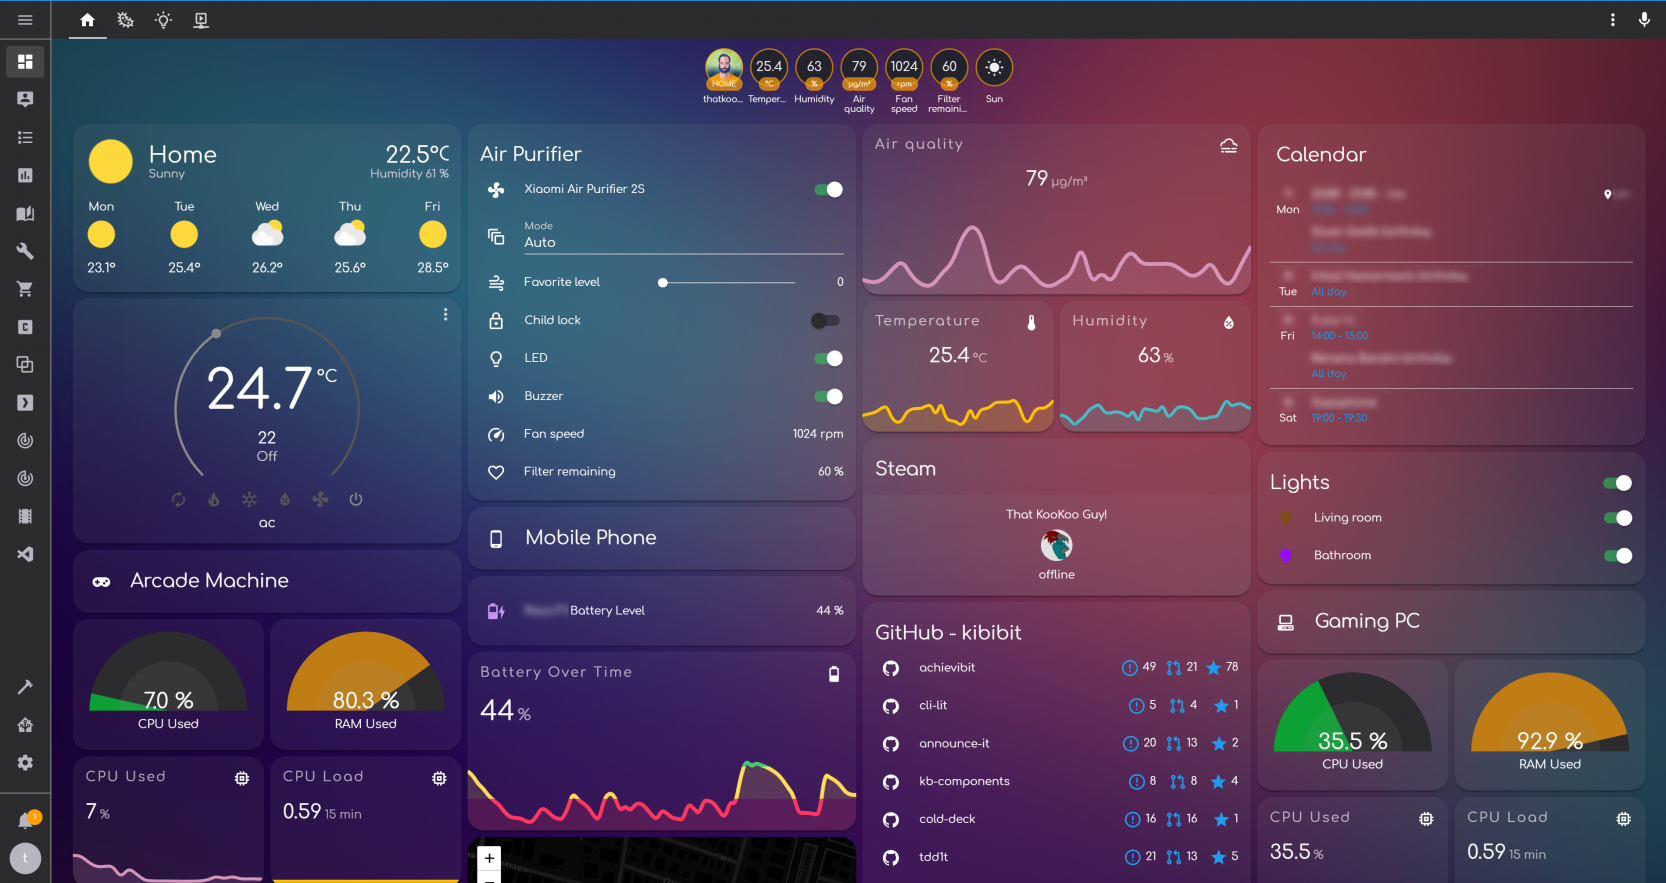
\includegraphics[width=\textwidth]{home_assistant}
	\caption{Interfața meniului principal, temperatură, grafice, consum energie.}\url{https://rbx.dk/w/home-assistant/hvad-er-home-assistant.html}
	\label{fig:home_assistant}
\end{figure}

\section{Apple Home}

Apple este una dintre primele companii care au încercat să integreze controlul casei smart într-o aplicație mobile, lansând HomeKit (Figura 1.2) integrat în IOS 8 care a apărut în septembrie 2014.

Cu suport de peste 100 brand-uri de produse, printre care termostate, prize inteligente, lumini și jaluzele, utilizatorii de Mac, Iphone, Ipad își pot automatiza sarcinile, numite \emph{Scenes}(care pot fi separate pe zone), prin apăsarea unui buton din interfața ușor de înțeles sau pot opta pentru integrarea cu asistentul vocal Siri.

Cristopher Null\footnote{\url{https://www.techhive.com/article/579157/essential-homekit-guide.html}.} de la TechHive afirmă că procesul de instalare este impresionant, dar folosirea acesui program zilnic poate fi \emph{mediocră}, fiind clasificată ultima când vine vorba de control din cauza pierderii semnalului și eșuarea executării task-urilor. Speră ca aplicația să primească update-uri și noi funcționalități, interacțiunea sa cu Apple Home lăsând mult de dorit. Se poate observa numărul de 10 ori mai mic de dispozitive suportate față de Home Assistant, fiind o barieră destul de observabilă atunci când se pune problema extinderii către alte funcționalități.

\begin{figure}[h]
	\centering
	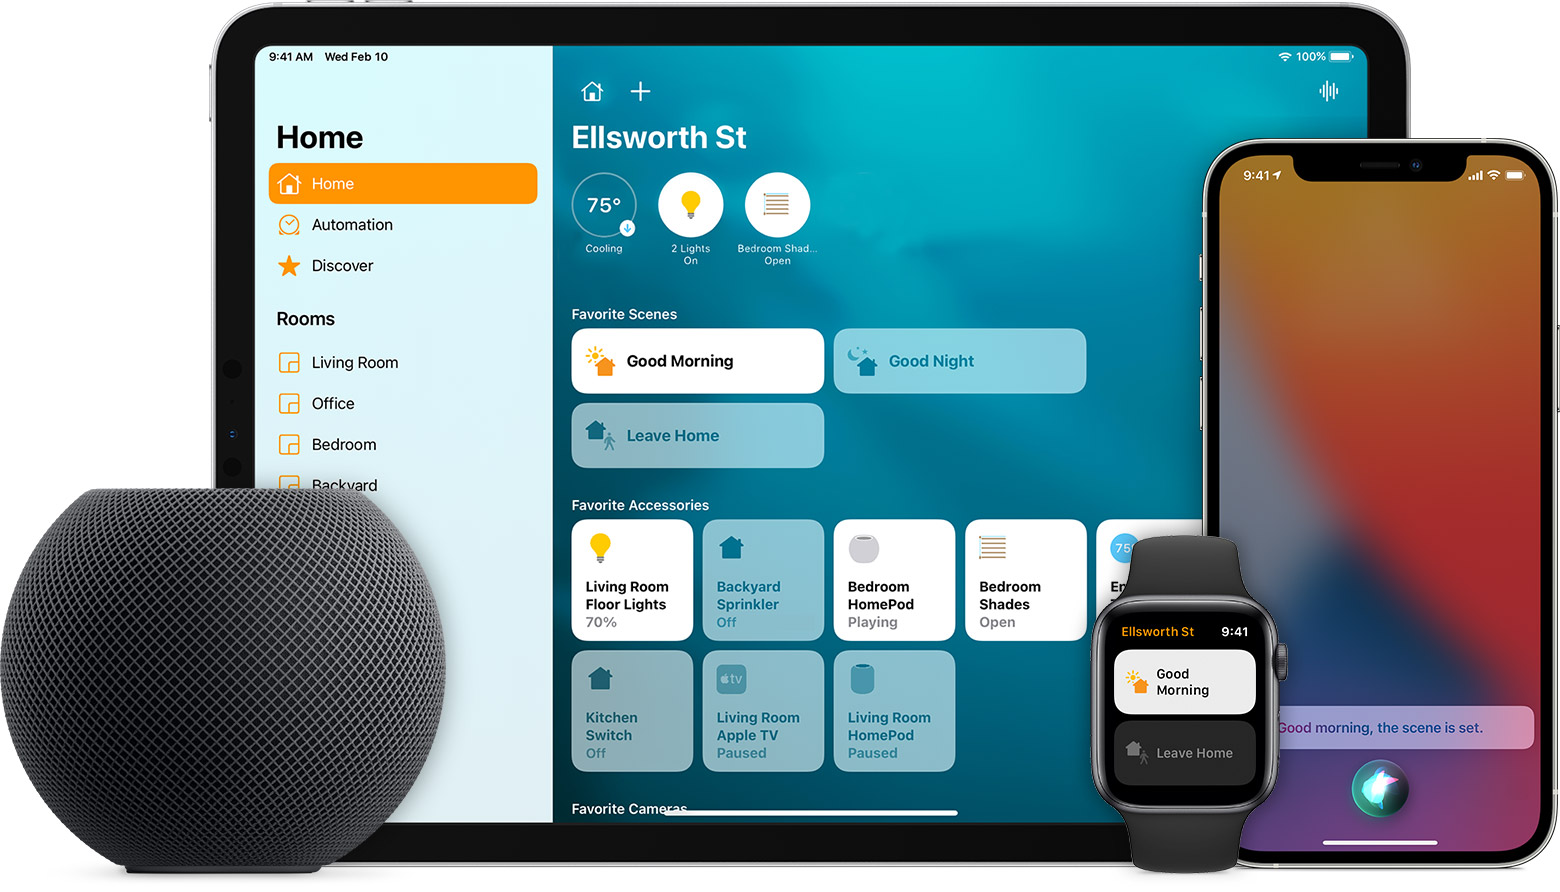
\includegraphics[width=\textwidth]{apple_home}
	\caption{Meniul principal împreună cu dispozitivele ce sunt în control.}\url{https://support.apple.com/en-us/HT208280}
	\label{fig:apple_home}
\end{figure} 


\section{IFTTT}

Fie că dorești să fii notificat pe telefon cu o zi înaintea unui eveniment sau că vrei ca asistentul Google să îți schimbe intensitatea luminilor din garaj, acestea sunt exemplele de bază pe care platforma \emph{IF this then that} (prescurtat \textbf{IFTTT}) (Figura 1.3) le poate realiza.

Acesta este un serviciu ce îți oferă posibilitatea de a conecta aplicații, servicii și dispozitive fără a fi preocupat de programarea lor. Website-ul IFTT și aplicația de telefon te ajută să construiești comenzi (pe care IFTTT obișnuia să le numească \emph{rețete}, acum sunt \emph{applets}) folosind card-uri colorate puternic pentru identificare.

Odată intrat pe pagina de start, se pot vedea applet-urile care sunt conectate cu ajutorul informațiilor de la capătul cardului. Pentru crearea unui astfel de item, trebuie specificat serviciul ce declanșează automatizarea respectivă. Odată ce se întâmplă acel trigger (\emph{if this}), se vor executa acțiunile definite de către utilizator (\emph{then that}). Ex: dacă ai adăugat o melodie nouă într-un playlist pe Spotify, adaug-o și pe Apple Music.


\begin{figure}[h]
	\centering
	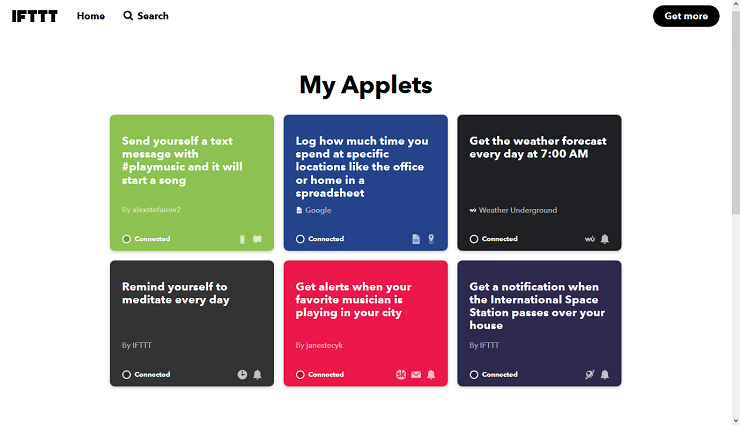
\includegraphics[width=1\textwidth]{IFTTT}
	\caption{Card-urile colorate pentru diferențiere, cu descriere, status și autorul informației.}\url{https://www.pcmag.com/reviews/ifttt}
	\label{fig:ifttt}
\end{figure}

\break
\hfill

\hfill

Prin intermediul ideilor prezentate precedent, putem observa că soluțiile pentru o casă smart sunt din ce în ce mai populare. Este foarte probabil ca un utilizator să dețină dispozitive IoT pe care le poate inter-conecta cu scopul de a obține o utilizare eficientizată a spațiului de lucru.

Soluțiile pentru o casă smart oferă oportunități diverse de a îmbunătăți controlul și automatizarea locuinței. Fiecare platformă are propriile caracteristici și avantaje, iar utilizatorii pot alege în funcție de nevoile și preferințele lor specifice.
    \chapter{Tehnologii utilizate}

\section{Flutter}

\textbf{Flutter} este o platformă pentru dezvoltare de aplicații publicată inițial în 2017. Cu ajutorul acestui \textbf{SDK} (\emph{Software Development Kit}), programatorii pot construi aplicații web, desktop și cross-platform pentru Android și IOS. Se folosește împreună cu limbajul de programare Dart.

Pentru a dobândi o eficiență asemănătoare celei native, este folosită compilarea \textbf{AOT} (\emph{ahead-of-time}) pe toate platformele în afară de Web, unde codul este convertit în JavaScript.

Fundația acestui SDK este scrisă în \textbf{C++}, oferă randare low-level folosind biblioteca \emph{Skia} de la Google sau un strat de abstractizare grafic \emph{Impeller}. Componenta de bază în Flutter este \emph{widget-ul} care poate conține și alte widget-uri. Acesta descrie logica, interacțiunea și design-ul unei componente UI. Flutter conține două pachete de elemente UI: Material Design (Google) și Cupertino (Apple).
\begin{lstlisting}[style=python, caption=Widget Scaffold]
return Scaffold(
	body: Column(
		children: [
			Text('Acest text va fi pozitionat'),
			Text('Deasupra acestui text'),
			],
		),
	);
\end{lstlisting}

\section{Flask}

Flask este un micro-framework web ușor de utilizat și flexibil, scris în Python. A fost creat cu scopul de a fi simplu și minimalist, oferind totodată funcționalitățile esențiale necesare pentru dezvoltarea rapidă a aplicațiilor. Acesta permite definirea de rute pentru a mapa cererile HTTP/HTTPS primite către funcții. Prin intermediul adnotărilor, se pot atribui funcțiilor URL-uri și metode HTTP/S specifice, permițând astfel aplicației să proceseze cererea în funcție de parametrii primiți.

Datorită abordării sale minimaliste și comunității active, Flask a devenit unul dintre cele mai populare micro-framework-uri pentru dezvoltarea aplicațiilor web în Python.

Figura 2.2 reprezintă un script ce expune o rută care returnează un paragraf HTML cu textul \emph{Hello, World!}.

\begin{lstlisting}[style=python, caption=Exemplu minimal de aplicație Flask]
from flask import Flask	
app = Flask(name)
@app.route("/")
def hello_world():
	return "<p>Hello, World!</p>"
\end{lstlisting}

\section{Raspberry Pi Zero W}

Raspberry Pi este o familie de calculatoare, de mărimea unui card de credit sau mai mici, care au revoluționat industria cu prețul accesibil de doar \$25 al primei plăci. În ultimii 5 ani, acestea au dobândit o atenție foarte mare în rândul comunității \emph{Do it yourself (DIY)} datorită spectrului larg de utilizări în proiecte digitale și IoT.

Comunitatea Raspberry a crescut mult și consistent. În momentul de față, în urma căutării "Raspberry pi projects", ne sunt returnate 47.2 milioane de pagini care conțin tutoriale despre imprimante 3D, sisteme de irigare, de luat vederi, ad-blocker pentru rețea și multe altele.

În contextul versiunii Zero W (Figura 2.1), avem disponibilă o placă de mărimea unui pachet de gume: 6.5 x 3 x 0.5 cm pe care poate fi instalat un sistem de operare bazat pe GNU/Linux numit Raspbian OS. Are un procesor single-core de 1GHz, 512 MB LPDDR2 RAM, iesire mini HDMI, două porturi micro USB, Bluetooth 4.0 și 2.4GHz 802.11n Wi-Fi.

Aspectul special al acestor computere constă în cei 40 pini \textbf{GPIO} (\emph{General purpose input-output}). Aceștia sunt folosiți pentru conectarea de senzori, fiind ușor programabili cu ajutorul limbajului Python, sau pentru audiențe tinere, Scratch.


\begin{figure}[h]
	\centering
	
\includegraphics[width=0.65\textwidth]{raspberrypi}
	\caption{Fața și spatele plăcii Raspberri Pi Zero W}\url{https://www.raspberrypi-spy.co.uk/}
	\label{fig:raspberrypi}
\end{figure}

\section{Microcontrollere folosite}

Un microcontroller (abreviat \emph{MCU}) este un circuit integrat care combină funcționalitate microporcesorului (de obicei aflat sub un radiator de aluminiu pentru disiparea căldurii) cu componentele periferice: module \emph{Input/output}, memorie și interfețe de comunicare cu alte module. Dețin mai mulți pini de tip analog, digital și \textbf{PWM} (\emph{Pulse Width Modulation}) pentru conectarea cu alte module

\break

\subsection{Arduino Nano}

Arduino Nano (Figura 2.2) este fratele mai mic al plăcii Uno cu care împărtășește majoritatea funcționalității: microcontroller ATmega328, 32KB memorie flash, viteză de 16MHz și 22 pini I/O.  Singurele diferențe sunt mărimea redusă și portul de USB mini. Este perfect pentru persoanele care doersc să învețe tainele electronicii și a programării, fiind potrivit pentru proiecte ce au constrângeri legate de spațiul disponibil.

\begin{figure}[h]
	\centering
	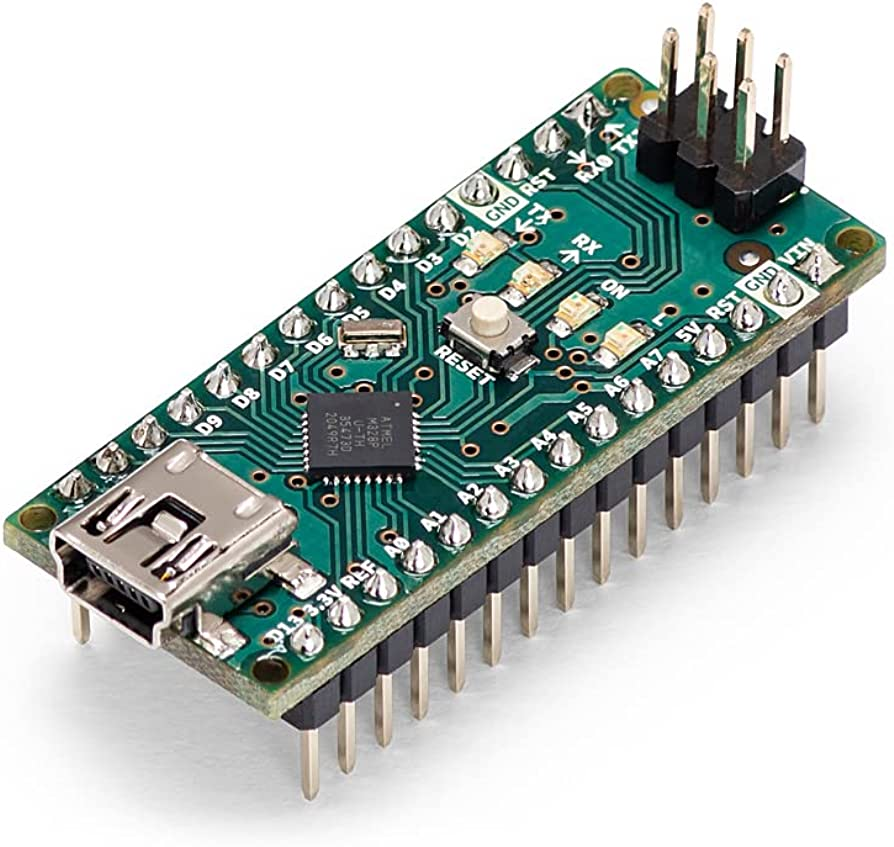
\includegraphics[width=0.4\textwidth]{arduino}
	\caption{Arduino Nano}\url{https://store.arduino.cc/collections/boards/products/arduino-nano}
	\label{fig:arduino}
\end{figure}

\subsection{ESP8266}

Modulul ESP8266 (Figura 2.3) este un \textbf{SOC} (\emph{System on a chip}) produs de firma Espressif Systems ce folosește stack-ul TCP/IP cu ajutorul căruia se poate conecta la internet.

Acesta a fost popularizat în anul 2014 de către alt SOC asemănător \textbf{ESP-01} al firmei \textbf{Ai-Thinker}. Chip-urile se pot conecta la rețele Wifi și să realizeze conexiuni prin utilizarea comenzilor de tipul \emph{Hayes}, \textbf{AT commands}.

La început, nu existau documentații în limba engleză. Dat fiind faptul că SoC-ul este ieftin și deține un număr mic de componente externe, acesta poate fi produs în volume mari la preț mic, ceea ce a atras mulți hackeri să-l exploreze și să traducă documentația. 

\begin{figure}[h]
	\centering
	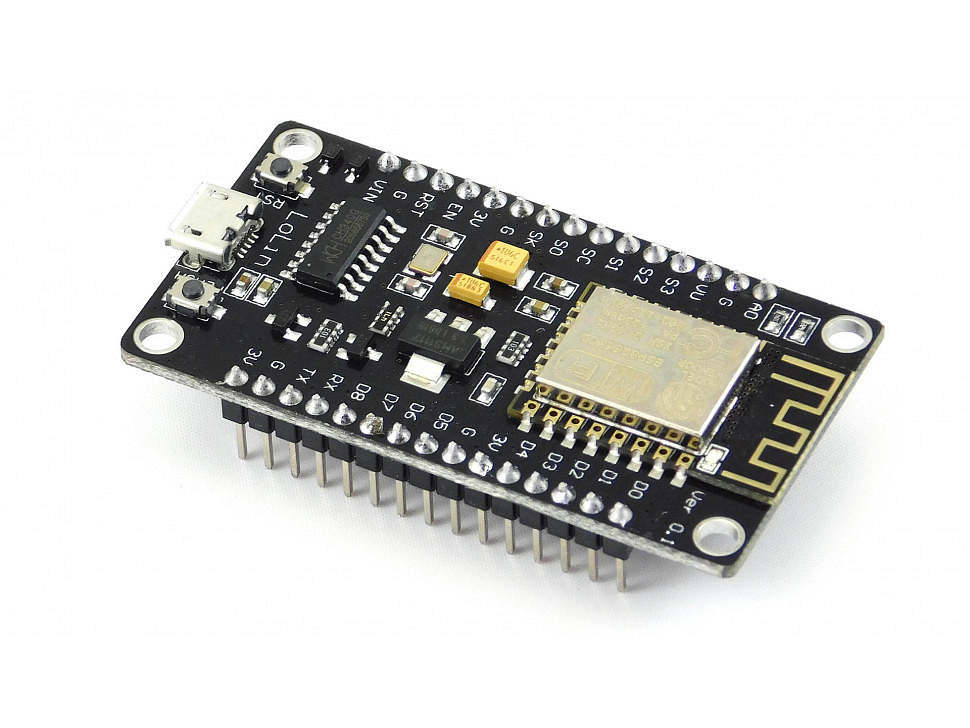
\includegraphics[width=0.5\textwidth]{esp8266}
	\caption{ESP8266 pe o placă \emph{Breakout}}\url{https://www.teachmemicro.com/esp8266-spiffs-web-server-nodemcu/}
	\label{fig:esp8266}
\end{figure}

\break

\section{Module} 

Modulul de comutare este echipat cu 2 relee (Figura \ref{fig:relay}) controlate individual. Acesta poate fi utilizat împreună cu orice placă de dezvoltare care dispune de 2 pini digitali și un pin VCC de 5 V. Produsul este util în multe proiecte de electronică în care trebuie controlate diferite dispozitive care sunt alimentate cu o tensiune maximă de 250 V AC sau 30 V DC.

Senzorul DHT22 (Figura \ref{fig:temperature}) este un senzor de umiditate și temperatură mic, ieftin și la îndemână. Folosește un senzor capacitiv de umiditate și un termistor pentru a măsura aerul din jur. Acesta oferă semnal digital pe pinul de date. Este ușor de folosit, dar este nevoie de atenție pentru citirea datelor la momentul potrivit.

Senzorul infraroșu HC-SR501 (Figura \ref{fig:motion}) este folosit pentru a detecta prezența oamenilor. Este des utilizat în aprinderea sau stingerea automată a luminii într-o încăpere atunci când o persoană ajunge sau părăsește o incintă. Suportă o tensiune de alimentare mai ridicată (5 – 20 V ) și are un consum mai mare. Are o rază de sensibilitate de 110\textdegree și detectează obiecte până la o distanță de 7m.

Placa HC-SR04 (Figura \ref{fig:distance}) deține un emițător și un receptor ultrasonic ce ne pot oferi distanșa până la cel mai apropiat obstacol într-un mod ușor de programat. E compatibilă cu o gamă variată de plăci de dezvoltare, având unele avantaje față de senzorii de distanță de tip analog: are nevoie doar de pini I/O digitali, are toleranță mai mare la zgomotul din circuit și precizie de până la 4.5 metri, toate la un consum continuu de maxim 2mA.

\begin{figure}[h]
	\centering
	\begin{subfigure}{0.3\textwidth}
		\centering
		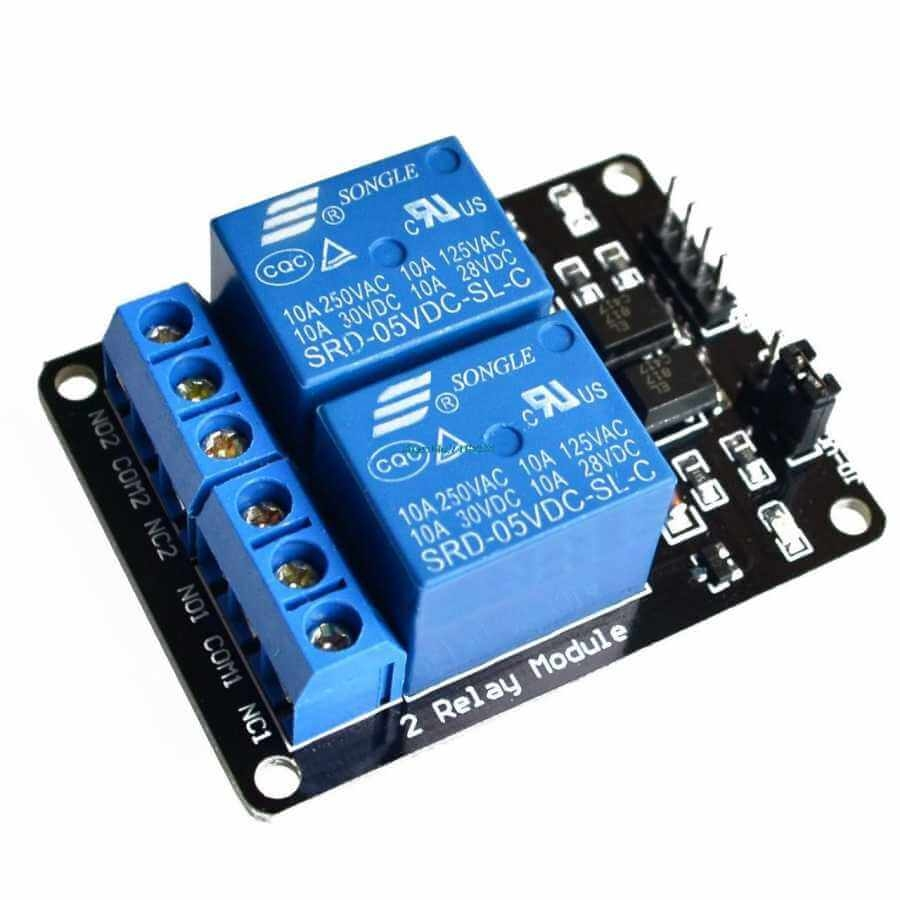
\includegraphics[width=\linewidth]{relay}
		\caption{Placă cu două relee pentru comutarea tensiunii prizei}
		\label{fig:relay}
	\end{subfigure}
	\hfill
	\begin{subfigure}{0.3\textwidth}
		\centering
		
\includegraphics[width=\linewidth]{temperature}
		\caption{Senzor de temperatură și umiditate}
		\label{fig:temperature}
	\end{subfigure}
	
	\begin{subfigure}{0.3\textwidth}
		\centering
		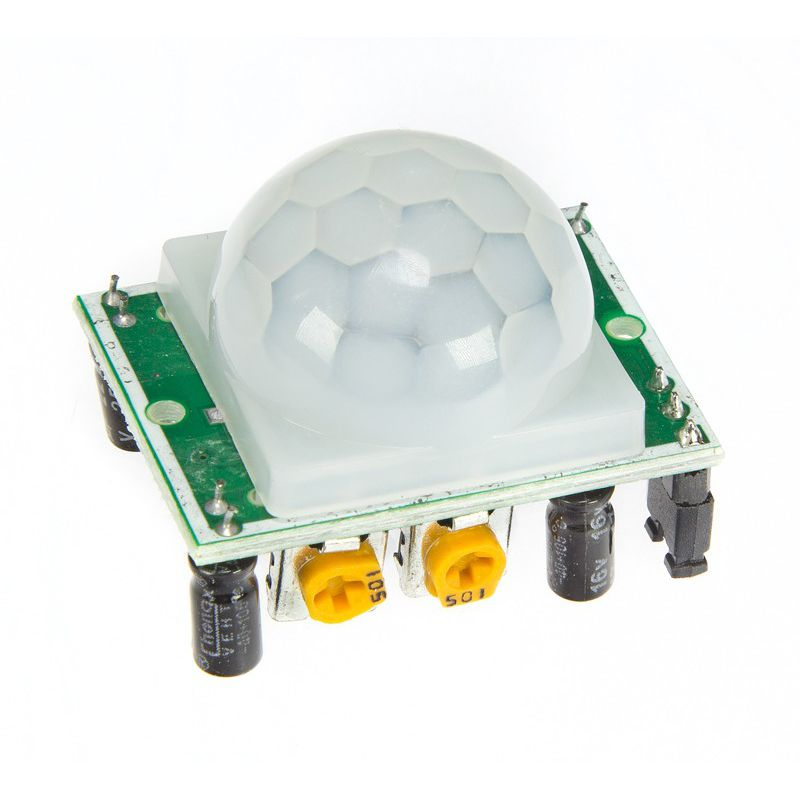
\includegraphics[width=\linewidth]{motion}
		\caption{Senzor de detectare a mișcării}
		\label{fig:motion}
	\end{subfigure}
	\hfill
	\begin{subfigure}{0.3\textwidth}
		\centering
		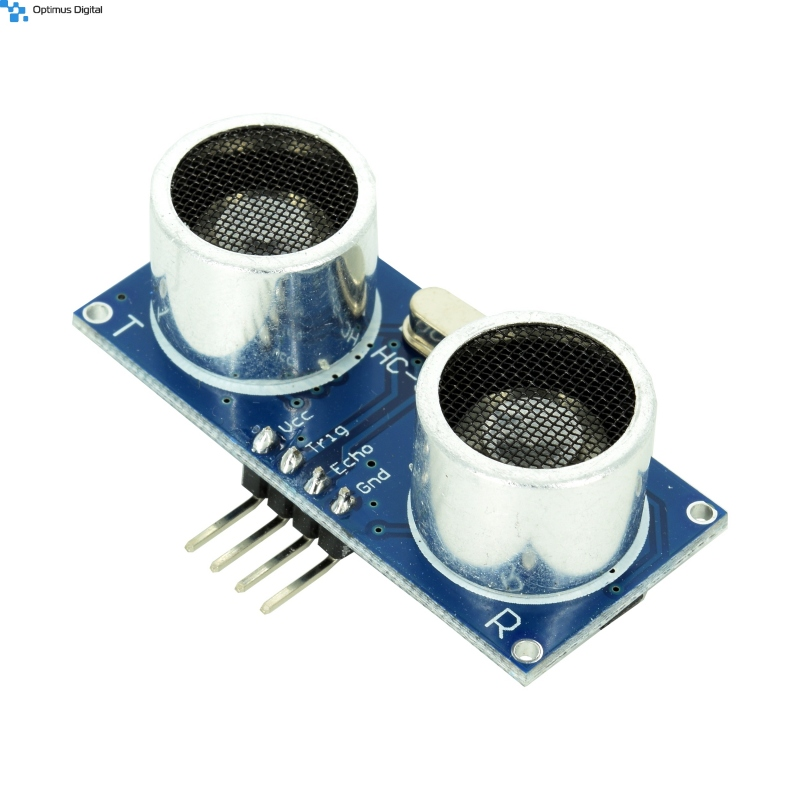
\includegraphics[width=\linewidth]{distance}
		\caption{Senzor de măsurare a distanței}
		\label{fig:distance}
	\end{subfigure}
	
	\caption{Senzorii folosiți în acest proiect}
	\label{fig:all}
\end{figure}
\section{Motivatia tehnologiilor folosite}

Domeniul Smart Home este foarte vast și oferă o gamă largă de oportunități creative. Tehnologia a evoluat rapid, permițând controlul și automatizarea diverselor aspecte ale locuinței, de la iluminat și securitate la gestionarea energiei și confortul locatarilor. 

Modulele și plăcile utilizate se pliază pe arhitectura aplicatiei implementate, dar cum tehnologia avanseaza pe zi ce trece, va exista posibilitatea ca in viitor sa apara device-uri care pot creste performanta. Prin urmare, în domeniul caselor inteligente, nu există limite, iar utilizatorii sunt încurajați să-și folosească imaginația și să exploreze noi soluții ce se pliază vieții personale.
    \chapter{Titlul celui de-al treilea capitol}

Amet venenatis urna cursus eget. Quam vulputate dignissim suspendisse in est ante. Proin nibh nisl condimentum id. Egestas maecenas pharetra convallis posuere morbi. Risus viverra adipiscing at in. Vulputate eu scelerisque felis imperdiet. Cras adipiscing enim eu turpis egestas pretium aenean pharetra. In aliquam sem fringilla ut morbi tincidunt augue. Montes nascetur ridiculus mus mauris. Viverra accumsan in nisl nisi scelerisque eu ultrices vitae. In nibh mauris cursus mattis molestie a iaculis. Interdum consectetur libero id faucibus nisl tincidunt eget. Gravida in fermentum et sollicitudin ac orci. Suscipit adipiscing bibendum est ultricies. Etiam non quam lacus suspendisse. Leo urna molestie at elementum eu facilisis sed odio morbi. Egestas congue quisque egestas diam in arcu cursus. Amet consectetur adipiscing elit ut aliquam purus.

\section{Titlul secțiunii 1}

Eros donec ac odio tempor. Facilisi morbi tempus iaculis urna id volutpat. Faucibus in ornare quam viverra orci sagittis eu. Amet tellus cras adipiscing enim eu turpis egestas. Integer feugiat scelerisque varius morbi. Platea dictumst vestibulum rhoncus est pellentesque elit ullamcorper dignissim. Bibendum arcu vitae elementum curabitur. Eu nisl nunc mi ipsum faucibus. Id aliquet lectus proin nibh nisl condimentum id venenatis a. Cras adipiscing enim eu turpis egestas pretium. Quisque non tellus orci ac auctor augue mauris augue. Malesuada pellentesque elit eget gravida cum. Ut lectus arcu bibendum at. Massa id neque aliquam vestibulum morbi blandit. Posuere ac ut consequat semper viverra nam. Viverra adipiscing at in tellus integer feugiat scelerisque varius morbi. Morbi enim nunc faucibus a pellentesque sit amet porttitor eget. Eu feugiat pretium nibh ipsum consequat nisl vel. Nisl purus in mollis nunc sed.

\section{Titlul secțiunii 2}

Elementum sagittis vitae et leo duis ut diam quam nulla. Purus sit amet volutpat consequat mauris nunc. Tincidunt augue interdum velit euismod in pellentesque massa. Nunc sed augue lacus viverra vitae congue. Porttitor leo a diam sollicitudin. Faucibus pulvinar elementum integer enim. Adipiscing bibendum est ultricies integer quis auctor elit. Blandit aliquam etiam erat velit scelerisque in. A iaculis at erat pellentesque adipiscing commodo elit at. Erat nam at lectus urna duis. Consequat ac felis donec et. Fermentum posuere urna nec tincidunt praesent semper feugiat nibh sed. Proin gravida hendrerit lectus a. Pretium viverra suspendisse potenti nullam ac tortor vitae purus. Arcu cursus euismod quis viverra nibh cras pulvinar mattis. Gravida arcu ac tortor dignissim convallis aenean. Quam nulla porttitor massa id neque aliquam vestibulum morbi. Sed viverra ipsum nunc aliquet. Quis enim lobortis scelerisque fermentum dui faucibus in.
    \chapter{Scenarii de utilizare}

În acest capitol vor fi prezentate 4 scenarii în care un utilizator ar putea folosi aplicația, oferind un ghid clar despre modul utilizării fiecărui procedeu.

\section{Colectare de date și logging}

Funcționalitatea de bază a acestei soluții este de a citi valorile curente ale fiecărui senzor pentru a fi stocate în baza locală de date.

Utilizatorul dorește să verifice statutul fiecărui device din locuința sa. Acesta deschide aplicația de telefon, trece de splash-screen și îi sunt afișate toate cartonașele senzorilor conectați la stația de bază. La prima vedere, se poate observa doar ultima înregistrare, dar dacă user-ul dorește să vadă graficul ultimelor citiri, trebuie să apese pe cartonașul specific curiozității sale și să selecteze mărimea eșantionului dorit, astfel fiindu-i prezentate datele necesare. 

\section{Comutarea luminilor din holul intrării}

Înainte de a ajunge acasă, utilizatorul intră în aplicație și dezactivează modul de securitate. După ce acesta intră pe hol, luminile din încăpere se vor aprinde automat datorită senzorilor care au detectat mișcarea, rămânând aprinse pentru toată perioada cât utilizatorul nu a părăsit încăperea. 

În cazul în care utilizatorul a configurat și alte comutatoare (lumini, jaluzele smart, termostat), acțiunile dorite pot fi accesate din pagina dedicată senzorului respectiv și apăsând pe butonul ce reprezintă cerințele persoanei.

\section{Detectarea problemelor în comunicare}

Fiind un proiect de tipul \emph{Do it yourself}, utilizatorul trebuie să își configureze fiecare senzor, de la programare până la alimentarea constantă. În timpul acestui proces, user-ul observă că unul din senzori nu apare pe interfața mobilă, așa că:
\begin{itemize}
	\item se loghează prin \emph{ssh} la stația de bază pentru a executa scriptul de debug și
	\item deschide \emph{Serial Monitor} din \emph{Arduino IDE}.
\end{itemize}

Acesta citește erorile care sunt afișate la linia de comandă și remediază problema.

\section{Generarea raportului}

Utilizatorul este victima unei intruziuni în casă din cauza faptului că nu a verificat aplicația de telefon pentru eventualele anomalii semnalate de senzori în modul de securitate. 

Persoana în cauză intră în aplicație, la secțiunea \textbf{Report} și introduce intervalul aproximativ al timpului intruziunii, urmând ca pe telefonul său să fie descărcat un fișier ce conține toate datele senzorilor: valoare și timpul ciritii, fișier ce ulterior va fi oferit investigatorilor și poliției.
    
    \chapter*{Concluzii finale} 
\addcontentsline{toc}{chapter}{Concluzii}

Lucrarea "Home Smartify - soluție pentru controlul dispozitivelor și securitatea casei" încearcă să ușureze modul de viață al utilizatorului, reușind să minimizeze legătura dintre acesta și dispozitivele pe care le are în casă. Aceasta este posibilă datorită aplicației de mobil pe care o poate folosi să își controleze senzorii din orice parte a lumii. Peste 6 miliarde de persoane folosesc un telefon mobil\footnote{\url{https://www.oberlo.com/statistics/how-many-people-have-smartphones}}, făcându-l un prim candidat când vine vorba despre modul în care utilizatorul să își controleze casa.

Cererea de soluții de tipul Smart Home este în continuă creștere. În anul 2022 numărul de case smart a crescut cu 14\%\footnote{\url{https://todayshomeowner.com/smart-home/guides/smart-home-facts-and-statistics/}} datorită 

\section{Direcții pe viitor}

Consider că proiectul poate fi îmbunătățit în mai multe arii. O primă remediere ar fi înlocuirea plăcii Raspberry Pi Zero W cu placa Raspberry Pi 4 deoarece procesorul cu un singur nucleu al primei plăci nu poate face față unui val de cereri API. Nucleele adiționare vor crește viteza de procesare a datelor care sunt citite de la senzori și vor scădea timpul de așteptare între cererile făcute de către telefonul utilizatorului.

Un alt punct de îmbunătățire ar fi modulul de transmitere al datelor senzorilor statici.

Un alt punct ce ar putea fi corectat ar fi afișarea celor mai recente informații din baza de date fără ca utilizatorul să fie nevoit să apese pe butonul de reîmprospătare. Acest lucru este posibil ca la fiecare citire recent introdusă în baza de date, serverul să notifice fiecare telefon de acest lucru și să trimită informațiile actualizate.

Nu în ultimul rând, aș hosta serverul în cloud pentru ca alți utilizatori să poată folosi această tehnologie smart.
    \chapter*{Bibliografie} 
\addcontentsline{toc}{chapter}{Bibliografie}

\begin{itemize}
    \item Author1, \textit{Book1}, 2018
    \item Author2, \textit{Boook2}, 2017
\end{itemize}
\end{document}
